\documentclass[journal]{IEEEtran}
\usepackage{graphicx}
\begin{document}

\title{Operating System and Applications Multi-Core Scalability Issues}

\author{Edward~Hills}

% make the title area
\maketitle

\begin{abstract}

Multi-core scalability is in the fore-front of every programmers mind when programming operating systems or any serious application programs. For a number of years now it has been impossible to increase a single cores clock speed due to several limitations, mainly heat and power consumption. This is why a new paradigm has arisen in which we put more and more cores into a single CPU. The next decade is expected to herald 100s or 1000s of cores on a single chip. This is why we must begin to start thinking about how we can scale our operating systems and applications to gain the full benefit of multi-core. This paper will talk about some methods to attack scalability as well as propose some new ideas.

\end{abstract}

\section{Introduction}
\IEEEPARstart{S}{calability} is an important issue in todays modern operating system era. Current operating systems (OSs) are being retro-fitted with techniques to increase their scalability. On a whole things are improving, and this can be seen in the versions of the Linux kernel which are being released. However, some researchers see this is a stop-gap rather than a solution. This is due to a number of factors which cannot simply be fixed to be more scalable due to their semantics. Some scalability issues include:

\vspace{2mm}

\begin{itemize}
\item Global or coarse-grained locks
\item TLBs
\item Shared Memory
\item Semantic Serialization
\item Cache misses
\item Unnecessary Resource Sharing
\end{itemize}

\vspace{5mm}

Coarse-grained locks are a major scalability issue in multi-core or even highly threaded systems. A coarse-grained lock is one that locks a larger area than it possibly needs to to accomplish a job that needs to run without interference or the possibility of a race condition. Original linux kernels had whole kernel global locks but these were quickly removed with smaller finer-grained locks, however these locks are still not fine enough in a multi-core environment.

TLB or Translation Look-aside Buffer holds a table of physical addresses as generated from the virtual addresses, these are needed to be global so that each core gets the same data, when updating or viewing the TLB a look must be held which stops all other processes from accessing it, for such a widely used data structure this can severely limit scalability.

Shared Memory is simply a region of memory that is shared amongst different cores, this can cause a range of problems which are discussed later.

Semantic serialization is the problem in which some code blocks must be run in serial just to the nature of their task, these are one of the hardest problems to overcome and the semantics need to be rethought and designed to remove these.

Having one core read what another core just wrote imposes a wide range of cache misses, if the same core that did the writing did the reading than it would be able to access it from cache and save on roughly 200 cycles to get it from memory.

Unnecessary resource sharing often occurs as side effects of bad programming or lack of thinking about scalability. Some resources simply do not need to be shared and we will see examples of this later.

Throwing more cores or processors at a problem may not be the ultimate solution however, as Amdahls Law \cite{Amdahl} shows, we are limited by the sections which must be run in serial, if a program spends 1 hour out of 20 (95\%) executing serial code then Amdahls Law shows that we can only speed up computation by 20x. This is why serial parts must be rethought and redesigned to be parallelised.

In this paper I will talk about previous papers and the techniques which have helped overcome these problems such as \emph{sloppy counters} \cite{sloppy-counters}, use of \emph{Read-Copy-Update} \cite{RCU} techniques and OSs which have done a full re-think of the kernel design with scalability in mind such as \emph{fos} \cite{fos}.

** talk about your idea when you have one here **

\section{Related Work}

Multi-core CPUs have been around for over a decade now and with this plenty of time to adjust and come up with ideas to help improve the scalability issues that we face. This section will discuss some issues and previous solutions to overcome these, as well as some new designs or ways of thinking about the issue of scalability. 

\section{Current OS Solutions}

Without changing drastically the way we think about modern operating systems we have no choice but to examine areas of the kernel we have now and find ways to limit the amount, what, where and when we share resources among each thread or core. By reducing the amount of sharing we have to do and by keeping everything as modular as we can, we can try and curb the amount of differing cores that must access the same thing. By doing this, we can improve scalability drastically. 

\subsection{Sloppy Counters}
\emph{Sloppy counters} proposed by Byord-Wickizer \emph{et al.} is a way of doing \emph{lazy updates}. The linux kernel uses shared counters for a range of tasks such managing resources and garbage collection, this a scalability issue if many cores are accessing an updating these counters. \emph{Sloppy counters} aims to remove this bottleneck by having each core have its own counter and update that instead of the shared counter. It does this in the hopes that it can keep spare references that new threads can use. It will have to reconcile with the central counter if the local count grows above a threshold value or when deciding whether an object should be deallocated, thus it is best used when objects are rarely deallocated.  

Sloppy counters has the added benefit of being backwards compatible with other kernel counters meaning that not all sections of the kernel need to be changed by only that which imposes scalability issues. However one down side is that that they use space proportional to the number of cores present.

By adding sloppy counters to keep track of \emph{dentrys}, \emph{vfsmounts}, \emph{dst\_entrys} and to keep track of memory allocated by TCP and UDP network protocols. 

One downfall of this paper \cite{sloppy-counters} is that it does not give specific quantifiable results when using just sloppy counters, this is because the paper benchmarks a range of applications with more than one improvement made to it.

\subsection{Read-Copy-Update}
Read-Copy-Update provides a solution to many scalability issues, an important one being contention in the address space design \cite{Bonsai}. Clements \emph{et al.} re-designed the address space to use a balanced binary tree, \emph{Bonsai}, to ensure non-destructive updates of the table.

I will now briefly describe RCU and how it helps with scalability in a multi-core environment.

The main idea of RCU is that when a reader process or thread comes to read a particular block thats inside an RCU synchronization block it first copies the data that is held within the data-structure and then makes a copy of the original pointer itself. Next, it simply carries on and if need be it updates its copy. It then updates the global pointer and waits a certain grace period. It has this grace period so that all other readers which are reading the original data-structure have time to finish. 

Once the code enters a 'quiescent state' (an area in the code in which you can guarantee that all previous operations have completed) then the grace period ends and the resource is reclaimed. There are several things that defines what a 'quiescent state' is, some methods simply use a counter and increment every time an operation is begun and decrement it when an operation is finished, then when the counter reaches zero it has completed everything before it. For non-preemptive systems if a context switch is performed then that could be classed as a quiescent state also. In some systems if an interrupt is called or a trap has been executed then these are also accepted.

RCU in its standard implementation is mainly for read-mostly data structures such as a routing table which is more often read than updated. One major advantage to RCU is its low-cost and low-overhead compared to normal synchronization techniques (such as a spinlock) which is relatively quite expensive and multi-processor unfriendly.

RCU is described as a 'two-phase' locking mechanism, the first phase is to carry out enough of each up-date for new operations to see the new state, but still let old operations carry on and the second phase is to finish the update once the grace period has finished.

RCU is a severe advantage over traditional locking mechanisms such as spinlocks as they are severely limited by worst-case memory latency. This is because once a traditional lock has been obtained it must write to the locked data-structure, this means that it must hit memory which is slow compared to cpu or cache.

There is a limitation however due to the \emph{wait\_for\_rcu()} function not working in a pre-emptible kernel unless pre-emption is specifically disabled for that section.
When implementing FD management with the use of RCU, Mckenney \emph{et al.} \cite{RCU} found that the kernel exhibited over 30\% more throughput for 4 cores and even with a uniprocessor there was a slight increase in performance (0.65\%).

Multi-core oriented OSs such as K42 use RCU pervasively as an existence lock. It is commonly used in Linux kernels since 2.5.

Read-Copy-Update locking technique allows multiple threads and cores to access the same data-structures without having to attain a lock which would limit scalability. Now knowing about RCU we can explain how this was used to help increase scalability in a concurrent address space.

By applying RCU to a balanced tree \cite{Bonsai}, \emph{Bonsai} allows us to perform read operations in parallel with writes and avoid cache coherence traffic caused by read locks. \emph{Bonsai} avoids the race conditions of keeping the red-black tree balanced by its design.

By implementing \emph{Bonsai} into the linux kernel, applications such as \emph{Metis} and \emph{Dedup} can achieve near-perfect speed-up to 80 cores and the results of Clements \emph{et al.} showed that the scalability improvement was likely to keep on being beneficial with even more cores.

\section{Future OS Solutions}

Techniques like the ones I have described above can almost be seen as 'stop-gaps' to the scalability issues we face in modern operating systems. These are becoming more and more effective as we devise new techniques for increasing scalability, however there are some that believe a total rethink and redesign of operating systems needs to be done. Below I will talk about a couple of these.

\subsection{Factored Operating-System}

\emph{fos} or Factored Operating System \cite{fos}, is an operating system that has been designed with scalability at the forefront of the developers mind. Fos aims to be able to support future massively multi-core chips (1000+ cores) that are likely to be around in the next decade or so. It has done away with contemporary modern operating systems such as Linux and has instead been rethought and redesigned to work a lot like Internet servers do today.

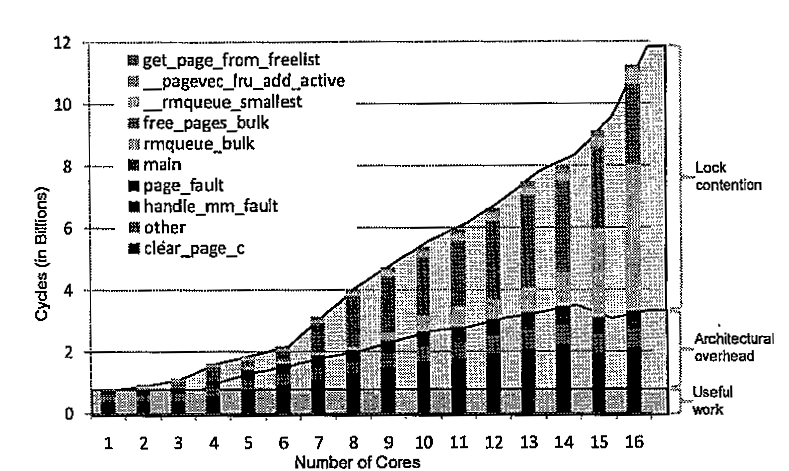
\includegraphics[width =9cm, height =8cm]{image.png}
The image above shows an interesting result which \cite{fos} discovered. The above is a graph of the physical memory page allocator and its ability to scale. You can clearly see that the more cores that are added the less 'useful' work is really done by the page allocator and the more time it spends waiting on locks. 

Fos takes its main fundamental idea from common Internet servers that are used everyday for the web. These servers are highly scalable and can deal with millions of users at a time. In a nutshell fos has a few separate and important ideas:

\vspace{2 mm}

\begin{itemize}
\item Kernel and Application code execute on separate cores
\item Each core performs a set of separate services
\item Main communication between cores is via message passing
\item Sets of services and applications can be broken up into multiple \emph{fleets}
\item Timesharing system replaced with spatial sharing
\end{itemize}

\vspace{5 mm}

By designing fos with the above view we instantly avoid the need for a majority of locks as well as avoided having the application and kernel interfere with each other. Below are just some of the benefits offered such as:

\vspace{2 mm}

\begin{itemize}
\item Inherently avoids contention between application and kernel
\item Only one thread for each core avoids locks
\item Quicker access to servives and fully parellised as tasks are spatially-shared not time-shared
\item Avoids expensive context switches
\end{itemize}

\vspace{5 mm}

The system service servers execute on top of a thin microkernel inspired by designs such as Mach \cite{Mach}, however there are a few differencnes such as distribution and parallelizing within a single system service server and having a spatially aware placement engine/scheduler. The lowest level of software management comes from the microkernel.

To describe further the relationship between fos and Internet Servers, fos even uses a cached namespace server (which provides fast lookup) and controls which messages get sent to which servers. This makes it possible for nodes to drop in and out (like the Internet) without losing important information because the name server will make sure it gets to where it needs to go and ensure at least one server takes the message. Messages are deposited into \emph{mailboxes}.

A typical server is designed to process a queue of requests, perform an action and send a reply. Servers are designed to be stateless, just like a lot of Internet services. This means that these are can be transaction-oriented and therefore requires no locking to stop threads updating memory. To further help scalability, servers aquire all resourced before the transaction starts and will only yield to the next transaction (fos is a non-preemptive system).

Due to fos being a message passing system there is no shared memory locks between cores so immediately a major scalability issue has been resolved. There is only ever one thread executing at a time on a server and there is no preemption therefore no locks are needed. To avoid sharing hardware structures such as caches and TLBs the OS servers operate on different to cores than that of applications. The final major advantage is that different parts of the system are also spatially separated so do not implicitly interfere with shared data structures.  

There are few issues with fos however and that is that it now has a large amount of core-to-core communication, however this cost is vastly less than that of shared memory (15-45 cycles compared to about 200 cycles respectively). Another issue is that replacing traditionally shared data structures such as the file systems buffer cache may not be possible and is currently unknown whether a hardware or software solution will be best. Another major question is if there are no locks being used within or between servers if a sequence of transactions can occur without some rare race conditions happening.

As you can see from my \emph{brief} discussion of fos above that it offers a new and \emph{less-is-more} approach to scalability. It takes a design which we see everyday in our lives, the Internet. The server-client model has been shown to allow massively scalable approaches and this is what fos aims to acheive also. By separating the services and applications spatially across a massively multi-core processor traidtional operating techniques such as time-sharing is replaced. Fos is still in its developmental stage however but may be paving the way for future massively multi-core scalable operating systems.


\subsection{K42}
K42 blah

\section{New Proposal}

\subsection{Basic Idea}
My new idea to help improve scalability is to take a similar approach to that of \emph{fos} \cite{fos} and completely rethink the idea and design of the kernel. 

\subsection{Possible Implementation}

To implement the design I have discussed above I first though to blah blah blah

\section{Conclusion}
The conclusion goes here.
The conclusion goes here.
The conclusion goes here.
The conclusion goes here.

\bibliographystyle{abbrv}
\bibliography{asgn3}

% that's all folks
\end{document}

